\chapter{Développement de modèles}

Ce chapitre présente dans un premier temps l'approche de modélisation, puis traite un à un les modèles de la plateforme MASS.
Nous somme intéressé par mieux modéliser les consommations, et non pas par mieux modéliser le comportement des occupants

DIVERSITE DES OCCUPANTS: Les occupants se comportent différemment sous des conditions environnementales identiques. Les variables propres aux différents occupants comme l'âge ou le contexte familial peut impacter les comportement.

Dans la littérature les comportements sont étudiés comme un ensemble sans discrimination individuelle lors des suivis sur site. La distinction entre les occupants est alors perdue et seulement un occupant moyen est modélisé. Cela représente alors davantage un concept statistique que la modélisation de la diversité des comportements humains. Ainsi, le seul moyen de proposer des modèles qui rendent compte de la diversité des occupants est d'étudier les occupants individuellement au sein d'un échantillon d'individus suffisamment significatif.

\section{Collection de données}

\subsection{Suivi sur site}

\subsection{Enquêtes}

4.2.2 Da Yan, 2015

\subsection{Études de laboratoire}

\section{Développement de modèles}

Un bon modèle isole les meilleurs variables pour prédire un évènement ou un état



Afin de considérer au mieux les comportements des occupants du parc immobilier, nous proposons une approche qui permet de considérer la variété de contextes. Depuis quelques années le nombre de publications traitant du comportement des occupants n'a cessé de croître. La Figure \ref{fig:NbPerYear} montre l'évolution du nombre de publications en lien avec le comportement des occupants recensé par l'Annex66.  et la répartition des comportements 

\begin{figure}[h]
\centering
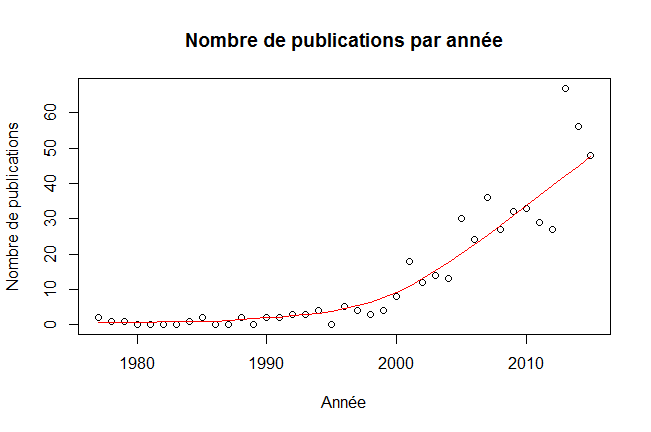
\includegraphics[scale=0.6]{Images/NbPerYear/NbPerYear}
\caption{Évolution du nombre d'articles publiés sur la modélisation du comportement des occupants}
\label{fig:NbPerYear}
\end{figure}

\subsection{Niveau de modélisation}

Le développement des modèles doit se faire avec parcimonie. La figure de principe \ref{fig:Fit-to-purpose} proposée par Pitt and Myung \cite{Pitt-02} met en garde sur la nécessité de développer des modèles qui sont ajustés aux objectifs de la modélisation. Un modèle sous-ajusté ne permet de reproduire le phénomène étudié, alors qu'un modèle sur-ajusté prendra en compte les variations non-significatives et ne sera pas reproductible. 

Gaetani et al. \cite{Gaetani-16} proposent une méthodologie, appelée \textit{fit-for-purpose} permettant de sélectionner le modèle le plus approprié à l'objectif de l'utilisateur. 

\begin{figure}[h]
\centering
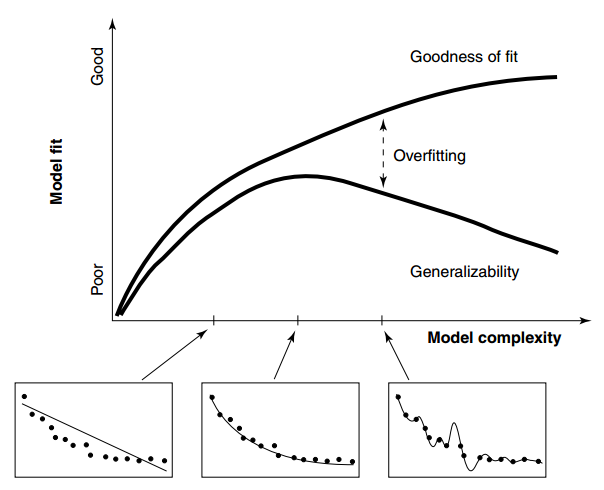
\includegraphics[scale=0.7]{Images/Model_fit}
\caption{Model fit}
\label{fig:Fit-to-purpose}
\end{figure}

\subsection{Famille de modèles}

\subsubsection{Modèles linéaires généralisés}

\subsubsection{Modèle de Bernoulli}

\subsubsection{Chaine de Markov}
\label{Chaine de Markov}

Une chaîne de Markov $\lbrace X_{t}:t=0,1,2,...n\rbrace$ est un processus stochastique capable d'estimer un état futur $X_{t+1}$ en fonction de l'état présent $X_{t}$ mais indépendamment des états passés $X_{0}, X_{1}, ...X_{t-1}$. Les chaînes de Markov ont alors l'avantage en comparaison avec le processus de Bernoulli de rendre la simulation davantage fiable sur les transitions d'états. La probabilité de transition d'un état $i$ au pas de temps $t$ à un état $j$ au pas de temps $t+1$ $(P_{ij})$ peut être formulé comme:

\begin{equation}
P(X_{t+1}=j|X_{t}=i)=:T_{ij}(t)
\end{equation}

On obtient alors la matrice de transition d'état $ T_{ij}(t)= \begin{bmatrix}
        T_{00}(t) & T_{01}(t) & \cdots & T_{0n}(t)\\
        T_{10}(t) & T_{11}(t) & \cdots & T_{1n}(t)\\
        \vdots & \vdots & \ddots & \vdots\\
        T_{n0}(t) & T_{n1}(t) & \cdots & T_{nn}(t)\\
     \end{bmatrix}$ pour $n+1$ états possibles.
     
Dans le cas d'un système binaire la matrice de transition $ T_{ij}(t)$ est réduite à 2 dimensions. La somme des probabilités d'une ligne étant égale à 1, il suffit de connaître deux probabilités de transition pour en déduire l'ensemble du système. La matrice réduite est donc $T_{ij}(t)= \begin{bmatrix}
        1-T_{01}(t) & T_{01}(t)\\
        1-T_{11}(t) & T_{11}(t)       
     \end{bmatrix}$

\subsubsection{Loi de Weibull}

\subsubsection{Approche hybride}

\subsubsection{Partitionnement de données}

\subsection{Évaluation et validation}


\section{Interaction sociales}
Ne pas présenter sous cette forme

Les interactions sociales ont lieu d'une part pour modifier les activités car certaines peuvent être partagées, comme regarder la télévision. D'autre part ces interactions peuvent également modifier les actions réalisées sur des systèmes, comme l'ouverture des fenêtres.

Le développement des modèles suivant s'intéressera également aux dynamiques sociales entre les occupants. L'influence de la famille ou des colocataires en terme de négociation et de régulation sera en outre étudiée.

Plessis et al. \cite{Plessis-14} introduisent la notion de confort du groupe qui est utilisée pour déterminer quel action le groupe choisi (ex: augmenter la température, ouvrir la fenêtre). En opposition aux actions individuels (adaptation de l'habillement, changement d'activité).

Schweiker \cite{Schweiker-16} a étudié les interactions entre les occupants et le bâtiments. Il a constaté que les occupants de bureaux partagés ont tendance à moins modifier leur environnement que les occupants de bureaux individuels. ------Read the paper-------

\subsection{Quantification des activités}

Dans le but de quantifier les activités, on défini une unité appelée unité de service. Cette unité est définie par occupant. L'unité de service d'un logement ou d'une zone pour une activité peut donc être déterminé par l'agrégation de l'unité de service pour tous les occupants du logement. Cette agrégation dépend de la nature des activités, elle peut être partagée ou additive.

Une nature d'activité partagée correspond à une activité réalisée ou profitant à deux occupants ou plus. Par exemple, l'activité regarder la TV est considérée comme partagée car plusieurs occupants peuvent profiter de la même unité de service. Une activité est dite additive si l'unité de service du logement est la somme des unités de service individuelle. Par exemple, l'activité de toilette corporelle est additive car réalisée seule. Le tableau \ref{tab:activité et unité de service} présente les unités de services et la nature des activités. Une activité partagée signifie quelle peut être partagé ou additive.

\section{Activités et présence}

A mettre ailleurs: Le traitement de l'ensemble des résultats issus des simulations sont traité grâce au langage R. Le point fort de R par rapport à un logiciel à menus déroulants est dans la possibilité de programmer une suite d'analyses successivement. Comme les autres langages, R possède des structures de contrôle proches des langages Java et C/C++.

Les scénarios de présence dans les bureaux et d'activités dans les logements constitue une entrée indispensable pour les modèles adaptatifs (gestion de température de consigne, fenêtres, stores et volets, éclairage) et non adaptatifs (utilisation d'appareils électriques, consommation d'eau chaude). Nous proposons donc dans ce chapitre de considérer deux familles de modèles de prédiction des activités, d'une part les présences et absences dans les bâtiments de bureaux et d'autre part les activités dans les logements. Cette distinction fondamentale pour l'ensemble des chercheurs \cite{Vorger-14}, \cite{Page-08}, \cite{Chapman-14} peut être vue comme un \textit{fit-for-purpose} dans le sens ou les modèles sont radicalement différents et n'ont pas de racines communes.

Bien que les horaires de travail et les horaire d'occupation des logements soient très corrélés pour l'ensemble de la population, les deux modèles présentés dans ce chapitre sont totalement indépendant. Nous justifions ce choix par une modélisation dans cette thèse à l'échelle du bâtiment. Une modélisation plus large à l'échelle du quartier ou de la ville impliquerait alors une approche ou les activités professionnelles et privées seraient dépendantes.

\subsection{Bureaux}

L'objectif de ce chapitre est de proposer un modèle qui reproduit plus fidèlement la présence de travailleurs de bureaux que les scénarios conventionnels couramment utilisés. Le modèle proposé dans ce chapitre est définit en pré-processus de la simulation, c'est à dire qu'il est connu pour l'ensemble de la simulation avant que celle-ci n'ai débutée. Ce choix se justifie par la non-nécessité, à priori, de connaître les variables environnementales pour définir les horaires de travail. La première partie de cette section présente un état de l'art des modèles stochastiques de présence dans les bureaux et plus particulièrement le modèle de Page et al. \cite{Page-08} qui est utilisé comme base. La seconde partie présente comment ce modèle développé sur des bureaux universitaires de chercheurs peut être également appliqué sur des bureaux de catégories professionnelles plus large. Enfin, une présentation des résultats de ce modèle et de ces sous-modèles est proposé.

\subsubsection{État de l'art}

Afin d'établir des modèles stochastiques réalistes de présence dans les bureaux pour associer une présence à des apports métaboliques et à des actions possibles plusieurs travaux ont été réalisés.

Le premier modèle probabiliste recensé dans notre bibliographie date de 1995 et a été développé dans le cadre du programme Lightswitch par Newsham et al. \cite{Newsham-95}. L'objectif du programme était de modéliser les actions des occupants sur l'utilisation des appareils électriques. Or comme nous le verrons dans la section \ref {Gestion de l'éclairage} cette utilisation est fortement dépendante de la présence des occupants, notamment s'ils viennent d'arriver dans la pièce, s'ils en sortent ou s'ils sont en période intermédiaire. Les auteurs ont alors dans ce contexte développé un modèle stochastique qui intégre une variabilité temporelle de présence. D'autres auteurs, tels que Yamagushi et al. \cite{Yamaguchi-03} et Wang et al. \cite{Wang-05} ont également développés des modèles de présence dans des bâtiments de bureaux. Ces deux auteurs ont utilisé des chaînes de Markov homogènes pour le développement de modèle. En comparaison au processus de Bernoulli, les chaînes de Markov ont l'avantage de rendre la dynamique de simulation plus riche par la prise en compte de l'état précédent pour prédire le nouvel état. Cela impact donc fortement le nombre de transitions qui est alors plus réaliste et donc plus fiable pour la modélisation de l'utilisation de l'éclairage, de la gestion des ouvertures ou encore de l'utilisation d'électricité spécifique. Pour leur part, Erickson et al. \cite{Erickson-09} ont utilisé les données collectées d'occupation de bureaux pour développer un modèle basé sur des lois Gaussienne multidimensionnelles aux périodes de transitions. Ce modèle a par la suite été intégré dans un modèle à base d'agents dans le but de prédire la mobilité dans le bâtiment. Cependant, les résultats montrent une faible reproduction des mesures, de l'ordre de 20 \%.

Comme évoqué en introduction le modèle de Page et al. \cite{Page-08} nous semble le plus approprié. En effet, ce modèle repose sur des donnés issues d'instrumentations sur 5 bureaux entre décembre 2001 et janvier 2006, a été validé en outre par Feng et al. \cite{Feng-15} et a été réutilisé par de nombreux auteurs tels que Robinson et al. \cite{Robinson-07} dans l'outil SUNtool permettant d'optimiser la conception des quartier urbains ou Vorger \cite{Vorger-14} dans sa plateforme permettant un couplage entre les comportements des occupants avec le logiciel de simulation dynamique Comfie+Pleides.

Comme toujours dans notre contexte, la modélisation de la présence des occupants dans les bureaux a vocation à être utilisée comme une donnée d'entrée aux modèles de comportement des occupants vis-à-vis de la gestion des stores, des fenêtres, de l'éclairage ou encore des consommation électriques, dans les outils de simulations thermiques dynamiques et non pas comme une finalité en soit.

Dans la suite, nous utiliserons le modèle de Page comme une base ajustable, car il est construit sur une campagne de mesure significative longitudinale de 4 ans. Certes seulement 5 bureaux semblables ont été instrumentés, mais ce modèle est le plus robuste de notre base bibliographique. Néanmoins, afin de le rendre applicable à une gamme de bâtiments et un type d'occupants plus large, nous proposons d'y ajouter des facteurs contextuels rendant l'ensemble plus flexible et plus approprié.

\subsubsection{Modèle de Page}

Comme nous venons de le voir, les chaînes de Markov permettent de reproduire des transitions d'états et donc de rendre la dynamique de simulation plus cohérente avec les présences et absences des occupants. La section \ref{Chaine de Markov} a présenté le fonctionnement de base des chaînes de Markov. Page et al. \cite{Page-08} ont proposé un modèle de transition d'état pour les bâtiments de type bureau utilisant des chaînes de Markov. Sur la base de mesures de présence dans 5 bureaux de l'Ecole Polytechnique Fédérale de Lausanne pendant 4 ans, Page et al. ont proposé des probabilités de présences heure par heure pour une semaine type, soit 168 (24*7) probabilités. 

Les probabilités de transitions $T_{ij}(t)$ sont calculés à partir des probabilités de présence et l'équation suivante est déduite simplement:

\begin{equation}
T_{11}(t)=\dfrac{P(t)-1}{P(t)}T_{01}(t)+\dfrac{P(t+1)}{P(t)}
\label{T110}
\end{equation}

Néanmoins, une information est manquante pour déterminer les valeurs $T_{01}$ et $T_{11}$ à chaque pas de temps. Les auteurs ont alors défini un paramètre de mobilité:

\begin{equation}
\mu(t)=\dfrac{T_{01}(t)+T_{10}(t)}{T_{00}(t)+T_{11}(t)}
\label{mu}
\end{equation}

Pour simplifier les entrées du modèle et le calibrer les auteurs ont fixé ce paramètre $\mu$ à 0.13. Nous pouvons noter que plus $\mu$ est grand plus la transition d'état est fréquente.
A partir des équations \eqref{T110} et \eqref{mu} on peut alors déterminer les quatre probabilités de transition pour chaque pas de temps:

\begin{itemize}
\item $T_{01}(t)=\dfrac{\mu-1}{\mu+1}P(t)+P(t+1)$
\item $T_{00}(t)=1-T_{01}(t)$
\item $T_{11}(t)=\dfrac{P(t)-1}{P(t)}\left[\dfrac{\mu-1}{\mu+1}P(t)+P(t+1)\right]+\dfrac{P(t+1)}{P(t)}$
\item $T_{10}(t)=1-T_{11}(t)$
\end{itemize}

Lors du pré-processus de la simulation, la présence est calculés à partir des équations ci-dessus, afin d'être utilisée à chaque pas de temps de la simulation. Pour ce faire, à chaque pas de temps un nombre aléatoire $rand$ compris entre 0 et 1 est généré puis comparé à la probabilité de transition $T_{01}(t)$ si l'occupant est absent et à $T_{11}(t)$ si l'occupant est présent. Si $rand < T_{01}(t)$ alors l'occupant rentre dans la pièce, sinon non, et si $rand < 1-T_{11}(t)$ alors l'occupant sort dans la pièce, sinon il y reste.

La table \ref{PPage} présente les probabilités de présence $P$, pour les lundis et pour les dimanches, issues des mesures sur les 5 bureaux du modèle de Page et al. \cite{Page-08}. Les probabilités de présence du lundi sont représentatives de celles des jours de travail, alors que les probabilités du samedi sont semblables à celles du dimanche. Les sorties du modèle de base sont présentés dans la section \ref{Facteurs contextuels} avec les variantes.

\begin{table}[H]
\begin{tabular}{|c|c|c|c|c|c|c|c|c|c|c|c|}
\hline 
Heure & 1 & 2 & 3 & 4 & 5 & 6 & 7 & 8 & 9 & 10  \\ 
\hline 
$P_{Lundi}$ & 0.021 & 0.021 & 0.021 & 0.021 & 0.021 & 0.021 & 0.021 & 0.025 & 0.250 & 0.422  \\ 
\hline 
$P_{Samedi}$ & 0.028 & 0.030 & 0.029 & 0.029 & 0.030 & 0.029 & 0.029 & 0.030 & 0.030 & 0.030  \\ 
\hline
Heure & 11 & 12 & 13 & 14 & 15 & 16 & 17 & 18 & 19 & 20 \\ 
\hline 
$P_{Lundi}$ & 0.309 & 0.377 & 0.187 & 0.375 & 0.426 & 0.396 & 0.375 & 0.432 & 0.084 & 0.070 \\ 
\hline 
$P_{Samedi}$ & 0.035 & 0.037 & 0.030 & 0.032 & 0.041 & 0.045 & 0.042 & 0.034 & 0.035 & 0.032 \\ 
\hline 
Heure & 21 & 22 & 23 & 24 & \cellcolor{lightgray}& \cellcolor{lightgray}& \cellcolor{lightgray}& \cellcolor{lightgray}& \cellcolor{lightgray}& \cellcolor{lightgray}\\ 
\hline 
$P_{Lundi}$ & 0.047 & 0.039 & 0.038 & 0.038 & \cellcolor{lightgray} &\cellcolor{lightgray} &\cellcolor{lightgray} &\cellcolor{lightgray} &\cellcolor{lightgray} & \cellcolor{lightgray}\\ 
\hline 
$P_{Samedi}$ & 0.027 & 0.024 & 0.021 & 0.021 &\cellcolor{lightgray} &\cellcolor{lightgray} &\cellcolor{lightgray} & \cellcolor{lightgray}&\cellcolor{lightgray} &\cellcolor{lightgray}  \\ 
\hline 
\label{PPage}
\end{tabular}
\caption{Probabilités de présence dans les bureaux pour les lundis et les samedis}
\end{table}

\subsubsection{Facteurs contextuels}
\label{Facteurs contextuels}

Une fois le modèle brut de Page et al. \cite{Page-08} reprit dans la plateforme MASS, nous comparons nos résultats issus d'une simulation d'un an, d'un occupant et au pas de temps de 5 minutes avec ceux des auteurs pour vérifier la bonne programmation. L'article présente lui des graphiques sur 4 des 5 bureaux, une stricte comparaison est donc rendue délicate par l'absence d'indicateurs quantifiés, ceux-ci sont donc estimés sur les graphiques.

%%%% Ajustement du modèle de base

Plusieurs observations nous amènent à proposer un ajustement du modèle de base. Celles-ci sont de deux types, d'une part les observations communes entre les codes mais en contradiction avec nos connaissances socioprofessionnelles. Et d'autre part, des différences suffisamment significatives, entre la base et le modèle codé dans MASS, pour être rapportées ici.

Le premier indicateur venant à l'esprit pour évaluer le modèle est la durée de présence dans les locaux. Dans l'article de Page et al. \cite{Page-08} une erreur apparait, la durée de présence hebdomadaire moyenne est donnée à 24 heures, alors que la durée de présence quotidienne est quant à elle aux alentours de 9 heures. Sur une base de 5 jours de travail nous aboutissons dons à une incohérence évidente d'un facteur proche de 2.  De notre côté, notre simulation nous amène à une durée moyenne de 3h49 sur les 5 jours travaillés, soit légèrement moins que la durée hebdomadaire du modèle de base.

La comparaison des profils de probabilités de présence, nous permet de constater une bonne reproduction globale, mais une présence semble t-il légèrement plus élevée les nuits dans notre cas. La Figure \ref{Chronogramme} est un chronogramme sur une année de simulation, les zones noires représentent les périodes travaillées et les zones grises les absences. Nous identifions clairement les matins et après-midi comme périodes principalement travaillées, mais nous pouvons surtout noter des présences régulières courtes les nuits et confirmer notre impression issue du profil de présence.

\begin{figure}[H]
\centering
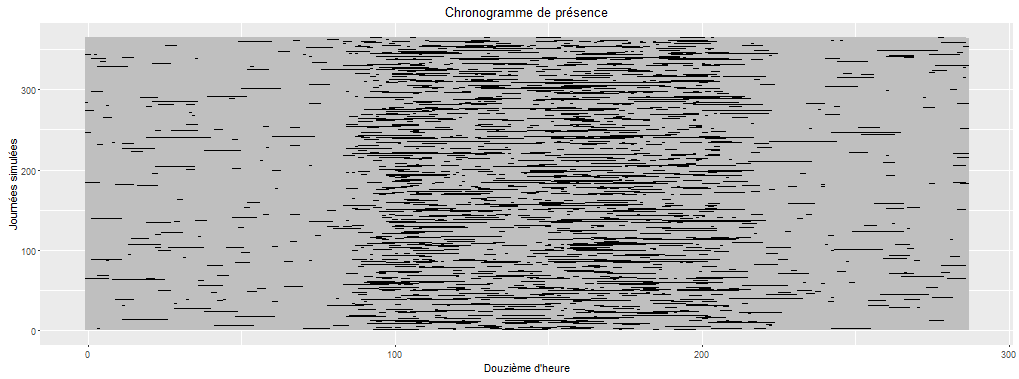
\includegraphics[scale=0.5]{Images/PageActivities/ChronogrammeBase}
\caption{Chronogramme de la présence d'un agent sur un an selon le modèle initial de Page et al \cite{Page-08}}
\label{fig:ChronogrammeBase}
\end{figure}



Sur la base d'une simulation d'une année, nous obtenons une moyenne d'heure de première arrivée dans les bureaux de 6h10 (une médiane de 7h20 et un écart-type de XX)

%%%%% Facteurs contextuels

Annex53

Pays, Salariés/Non-salariés, Extensif, Personnalisé

Type de bureaux


Nous avons démontré dans cette section que le modèle développé par Page et al. \cite{Page-08} peut être complété par l'intégration de facteurs contextuels, selon le type de bureaux ou selon la catégorie socioprofessionnelle. De plus, notre approche laisse également la possibilité au simulateur de définir lui même ses probabilités de présence s'il les connait. Nous avons testé cette solution en définissant les probabilités de présence suivante:
\begin{itemize}
\item en semaine de 0.8 \% de 8h à 12h puis de 13h à 17h, de 0,5 \% de 12h à 13h et de 0.05 \% sinon
\item le samedi de 0.05 \% toute la journée
\item le dimanche fermé toute la journée
\end{itemize}
 

\subsection{Logements}

Le fonctionnement général du modèle d'activités des logements est forcément très différent de celui des bureaux. Un point commun est qu'il est défini entièrement lors du pre-processus de la simulation. A la différence des bureaux, les activités dans les logements sont variées et ne sont donc pas limitées à la présence. Ces activités impliquent des comportements différents, des apports métaboliques différents dans les différentes zones du logement. La première partie de cette section présente l'état de l'art et plus particulièrement deux modèles qui nous ont interpellé et que nous avons opposé. La seconde partie porte sur la présentation détaillée du modèle de Jaboob \cite{Jaboob-16} répondant à nos exigences avec parcimonie. Le modèle idéal comporte un nombre de paramètres d'entrée limité, il rend compte de la diversité des activités en fonction du type d'habitants et produit des profils d'activités différents pour des individus semblables. Un modèle d'activités stochastique dans les logements convient alors parfaitement à la nature stochastiques des comportements humains.

\subsubsection{État de l'art}

L'état de l'art a permis de déterminer que l'ensemble des modèles d'activités proposés se base sur des enquêtes emploi du temps. Ces enquêtes se basent sur des échantillons de population larges (de l'ordre de 10000 participants) qui assurent une bonne représentativité des comportements de la vie quotidienne. Chaque répondant d'une enquête est associé à un descriptif socio-démographique et un carnet d'activités renseigné précisément sur une ou plusieurs journées. Le traitement de ces résultats permet de confronter les activités en cours avec les caractéristiques des individus. Ce traitement de données a mené à plusieurs modèles élaborés par Tanimoto et al. \cite{Tanimoto-08}, Widèn et al. \cite{Widen-12} ou encore Aerts et al. \cite{Aerts-14}, sans être exhaustif. Nous proposons dans la suite de détailler deux modèles qui ont particulièrement attirés notre attention, celui de Wilke et al. \cite{Wilke-13} et celui de Jaboob \cite{Jaboob-16}.

Vorger \cite{Vorger-14} reprend la stratégie de modélisation des activités dans les logements de Wilke et al. \cite{Wilke-2013}. La base de données utilisée est issue de l'étude de 1998-1999\footnote{L'Enquête Emploi du Temps (EET) n'est plus disponible en ligne et a été remplacée par l'enquête plus récente de 2009-2010} de l'INSEE sur 7949 ménages et 15441 individus français qui ont noté leurs activités sur une journée toutes les 10 minutes. Le modèle proposé issu de cet EET permet dans une première étape de générer pour chaque occupant des périodes de présence et d'absence. Lorsqu'une période de présence débute, une des 20 activités débute également, suivant un modèle de Markov, et une durée lui est attribuée, suivant une loi de Weibull. Si l'activité prend fin avant la période d'absence alors une autre activité débute. En revanche, si une période d'absence commence avant la fin de l'activité alors cette dernière est abrogée. Les modèles de Markov et Weibull sont influencés par l'heure de la journée, par des caractéristiques du ménage et par des caractéristiques individuelles des occupants, rendant les profiles d'activités très spécifique à chaque occupant. On peut néanmoins noter que ce modèle hybride présente quelques légers point d'amélioration à apporter. En effet, en raison de la non-continuité de l'enquête emploi du temps à minuit, les activités sont interrompus chaque jour à minuit conduisant à un début de période de sommeil quasi général à minuit et très rarement avant minuit. L'enquête datant de 1999, on peut également se demander si l'évolution des pratiques n'est pas suffisamment significative pour considérer une mise à jour. Aussi, le nombre de vingt activités renseignées nous semble excessif pour un exercice de modélisation de la performance énergétique.

Jaboob \cite{Jaboob-16} a plus récemment proposé un nouveau modèle d'activités basé sur une enquête emploi du temps anglaise datant de 2000-2001. La base de données est issue de questionnaires également renseignés toutes les 10 minutes sur une journée par 6500 ménages et 11700 individus. A partir de ces données, 10 modèles ont été développés et comparés. Il est conclu que le modèle de hybride Markov + Weibull fonctionne le mieux mais que le modèle de Bernoulli seul est recommandé pour sa simplicité et son faible nombre de paramètre d'entrées (240 contre 2880) tout en étant que très légèrement moins performant que le modèle hybride. Sur la base de ces conclusions, Chapman \cite{Chapman-16} utilise pour la prédiction des activités résidentiels ce modèle parcimonieux de Bernoulli, celui-ci ayant été recommandé. La qualité des modèles a été jugé en se basant sur 5 critères de validation et d'évaluation: 
\begin{itemize}
\item la sensibilité qui évalue la capacité du modèle à donner un résultat positif lorsqu'une hypothèse est vérifiée
\item la spécificité qui évalue la capacité du modèle à donner un résultat négatif lorsque l'hypothèse n'est pas vérifiée.
\item la précision qui regroupe la sensibilité et la spécificité
\item l'écart moyen à la moyenne, qui évalue l'amplitude de la différences de probabilité entre les simulations et les mesures.
\item l'indice de Brier, qui évalue la précision des probabilités du modèle
\end{itemize}

Or, nous notons qu'aucun de ces paramètres n'évalue le nombre de transitions d'état, qui nous semble pourtant fondamental pour reproduire des emplois du temps probables. Pour cette raison, il nous semble plus approprié d'utiliser un modèle d'activités hybride qui associe à chaque activité commencée une durée. Mahdavi et Tahmasebi \cite{Mahdavi-2014} proposent un indicateur, sans unité, qu'ils appellent erreur du nombre de transitions et qui est défini par le nombre de transitions prédit moins le nombre de transitions mesurées. Ne possédant pas la base de donnée utilisée par Jaboob pour le développement du modèle, nous proposons dans la suite de simplement calculer le nombre de transitions d'état par jour issu des modèles et de les comparer.

\subsubsection{Processus de Bernoulli}

A partir de l'EET Anglaise, Jaboob \cite{Jaboob-16} propose un modèle permettant de générer 10 activités. En pré-processus, le modèle calcule pour chaque pas de temps l'activité réalisée pour les occupants. La Table \ref{tab:Activités} les synthétise et associe à chaque activité le lieu où elles se produisent et l'état de l'occupant associé.

La diversité entre agents impacte leurs activités. Les variables explicatives des activités dans les logements sont relatives aux occupants (age, statut civique, genre, retraité/actif, chômeur/actif, niveau éducatif), au ménage (situation familiale, possession d'un ordinateur) et à l'environnement (heure de la journée, jour, saison). La Table \ref{VariablesActivité} détaille ces variables et leurs différents niveaux.

\begin{table} [H]
\centering
\begin{tabular}{|p{5 cm}||p{5 cm}|p{5 cm}|}
\hline Activités & Localisation & État de l'occupant (Clo et Met [$W/m^{2}$]) \\
\hline
\hline 0- Dormir & Chambre & Clo = 2.55 \newline Met = 46 \\
\hline 1- Passif & Salon & Clo = 1 \newline Met = 58 \\
\hline 2- Audio-visuel & Salon & Clo = 1 \newline Met = 70 \\
\hline 3- Bureautique & Bureau ou chambre & Clo = 1 \newline Met = 116 \\
\hline 4- Cuisine & Cuisine & Clo = 1 \newline Met = 116 \\
\hline 5- Nettoyage & Cuisine & Clo = 1 \newline Met = 116 \\
\hline 6- Toilette corporelle & Salle de bain & Clo = 0 \newline Met = 116 \\
\hline 7- Vaisselle et machine à laver & Cuisine & Clo = 1 \newline Met = 93 \\
\hline 8- Bricolage & Salon & Clo = 1 \newline Met = 93 \\
\hline 9- Absent & Extérieur & .  \\
\hline
\end{tabular}
\normalsize
\caption{Nature des activités et états associés}
\label{tab:Activités}
\end{table}

\begin{table} [H]
\centering
\begin{tabular}{|p{4 cm}||p{11 cm}|}
\hline Variables & Niveaux - \textit{Codes} \\
\hline
\hline Age & Plus de 59 ans - \textit{age1} \newline Entre 36 et 59 and - \textit{age2} \newline Moins de 36 ans - \textit{age3} \\
\hline Statut civique & En couple (marié, concubinage, partenaire civique) - \textit{civstat1} \newline Célibataire - \textit{civstat2} \\
\hline Genre & Homme - \textit{sex1} \newline Femme - \textit{sex2} \\
\hline Retraité & Actif - \textit{retired0} \newline Retraité - \textit{retired1} \\
\hline Chômeur & Actif - \textit{unemp0} \newline Chômeur - \textit{unemp1} \\
\hline Éducation & Lycée ou moins - \textit{edtry1} \newline Premier cycle - \textit{edtry2} \newline Second cycle et plus - \textit{edtry3}  \\
\hline Situation familiale & Adulte(s) sans enfants - \textit{famstat0} \newline Adulte(s) avec bébé (moins de 5 ans) - \textit{famstat1} \newline Adulte(s) avec enfants (entre 5 et 18 ans) - \textit{famstat2} \newline Adulte de plus de 40 ans sans enfants - \textit{famstat3} \newline Enfant avec parents ou garde - \textit{famstat4} \newline Enfant sans parents ou garde - \textit{famstat5} \\
\hline Possession d'ordinateur & Non - \textit{computer0} \newline Oui - \textit{conputer1} \\
\hline Heure & \textit{1 - 24} \\
\hline Jour & Lundi : Dimanche - \textit{day1} : \textit{day7} \\
\hline Saison & Printemps - \textit{season1} \newline Eté - \textit{season2} \newline Automne - \textit{season3} \newline Hiver - \textit{season4} \\
\hline
\end{tabular}
\normalsize
\caption{Variables sélectionnées pour expliquer les activités des occupants}
\label{VariablesActivité}
\end{table}

L'équation ci-dessous, issue de la régression logistique multinomial de l'EET, permet de calculer la probabilité, $P_{j}(x,t)$ de commencer une nouvelle activité.

\begin{equation}
P_{j}(x,t)=\frac{exp(A_{j}(x))}{\sum\limits_{j=1}^{N}exp(A_{j}(x))}, j = 1, .., N et A_{j}(x)= \alpha_{j}+\sum\limits_{k=1}^{n}\beta_{jk}x_{jk}
\end{equation}

N correspond au nombre d'activités total, soit 10, n correspond au nombre de prédicteurs, soit 10 (nombre de variables dans la Table \ref{VariablesActivité} excepté l'heure), $\alpha$ et $\beta$ sont respectivement l'interception et la pente. Les probabilités de commencer une activité dépendent ainsi des caractéristiques des occupants mais également du temps, en émane donc pour chaque occupant une matrice à 4 dimensions [10][24][7][4] (activités, heures, jour de la semaine et saison, respectivement).

\subsubsection{Modèle hybride}

Le modèle hybride couple au modèle de Bernoulli un modèle de Weibull. Ainsi, lorsqu'une activité débute, une durée correspondante y est associée. Wilke propose dans son modèle d'activités des coefficients de durée désagrégés. Bien sûr, les fonctions de Weibull diffèrent temporellement, la durée de l'activité de sommeil est plus longue si elle commence en début de nuit qu'en début d'après-midi, mais elle diffèrent également selon les caractéristiques des occupants, la durée d'un repas pour un retraité est plus longue que pour un actif. Pour considérer ces caractéristiques liées aux occupants les données sont structurées en arbres binaires. Pour chaque activité et chaque heure de la journée un arbre binaire est proposé, les nœuds de celui-ci étant formé par les attributs des occupants.

Au contraire, Jaboob \cite{Jaboob-16} fourni dans sa thèse les coefficients de forme et d'échelle de manière agrégés pour chaque heure et activité de la simulation, mais pas en fonction des caractéristiques des occupants. L'auteur justifie ce choix par un modèle davantage parcimonieux et une plus-value discutable de la désagrégation, les distinctions étant très peu intuitives et les caractéristiques des individus  multi-colinéaires. Pour ces raisons, nous décidons d'utiliser les coefficients agrégés de Jaboob.

La durée de l'équation est alors définie par l'équation ci-dessous, U étant un nombre aléatoire tiré entre 0 et 1. 

\begin{equation}
t_{j}=\frac{(-log(U))^{\frac{1}{k}}}{\lambda}
\end{equation}

Les paramètres de forme $k$ et d'échelle $\lambda$, déterminés par la méthode du maximum de vraisemblance, maximisent la probabilité de reproduire, par une loi de Weibull, la distribution observée de l'enquête emploi du temps.

Il est à noter que les coefficients de la loi de Weibull ne sont pas connus pour l'activité informatique (\textit{IT}) lorsqu'elle a lieu de 2 à 4 heures du matin dans la base de donnés de Jaboob. Cela est la conséquence d'un événement peu ou pas présent à ces heures dans la base de données. Pour s'affranchir de cette méconnaissance problématique pour le modèle, nous proposons une simple interpolation linéaire basée sur les intervalles de temps précédent et suivant:
\begin{equation}
f(x)=\frac{x_{b}-x}{x_{b}-x_{a}}y_{a}+\frac{x-x_{a}}{x_{b}-x_{a}}y_{b}
\end{equation}
Sachant que $\lambda(2)=61.806$ et que $\lambda(5)=40.125$ on a alors $\lambda(3)=54.579$ et $\lambda(4)=47.352$. Et sachant que $k(2)=1.143$ et que $k(5)=0.813$ on a alors $k(3)=1.033$ et $k(4)=0.923$. L'ensemble des coefficients se trouve en Annexe de la thèse de Jaboob \cite{Jaboob-16}.

\subsubsection{Présentation des résultats}

Afin de tester et visualiser les sorties des modèles d'activités dans les logements, nous avons généré un ensemble de graphiques, Figure \ref{fig:Activités}, qui présente les profils d'activités journaliers de 2 occupants différents, le premier est un jeune homme de 20 ans, avec ordinateur, actif et célibataire alors que le second est un retraité marié de 60 ans, sans ordinateur, sous les deux types de modèles, Bernoulli et hybride. Les profils générés par les deux familles de modèle sont globalement en accord avec le sens commun, nous pouvons néanmoins émettre un certain nombre de critiques. Pour la comparaison d'archétype, on retrouve sans surprise une proportion de temps à l'extérieur très supérieur chez l'occupant actif que chez le retraité, une durée devant la télévision supérieure pour le retraité ou encore une période de sieste plus significative chez les retraités. Étonnamment, plusieurs activités sont réparties uniformément sur la période d'éveil, comme l'activité cuisine dont on attendait des pics aux heures de repas. Également étonnamment, on note une importante proportion de l'activité informatique à 9 et 14 heure chez l'occupant retraité. Pour la comparaison des deux modèles on a tendance à penser que le modèle hybride reproduit mieux le sommeil que le modèle de Bernoulli qui génère assez peu d'heures de sommeil et un nombre d'autres activités semble t-il élevé. L'activité douche-toilette se retrouve dans le modèle hybride quant à elle réduite mais les deux pics du matin et du soir restent visibles.

La Figure \ref{fig:ExempleScenario} permet d'évaluer le nombre de transitions entre deux activités. Sans surprise, nous ne notons pas de différences significatives entre le nombre de transitions entre deux catégories d'occupants, au contraire du type de modèle. Sur 150 jours de simulations, le modèle de Bernoulli a généré en moyenne 185 activités quotidienne contre 56 pour le modèle hybride, pour un pas de temps de 5 minutes. Cet indicateur est difficile à interpréter rigoureusement car non comparable à une valeur étalon issue de la littérature ou de la base de données. En effet, l'enquête emploi du temps est à pas de temps fixe, plusieurs activités peuvent alors avoir lieu sur un même pas de temps sans être prise en compte dans l'enquête. Le nombre d'activités recensés dans l'enquête est également de grande influence sur le nombre de changement d'états. Enfin, le pas de temps de simulation, impacte considérablement ce nombre de transitions. Une simulation au pas de temps de 10 minutes a mené à 14 transitions, contre les 56 au pas de 5 minutes. Cet indicateur de nombre de transitions n'est en revanche pas sans intérêt, d'une part car il peut être utilisé pour comparer des modèles, ici le modèle de Bernoulli seul au modèle hybride Bernoulli (pour déterminer le début des activités) + Weibull (pour déterminer les durées des activités) et d'autres part pour mieux appréhender la dynamique des occupants dans ce modèle de prédiction des activités.

\begin{figure}[H]
\centering
\begin{tabular}{cc}
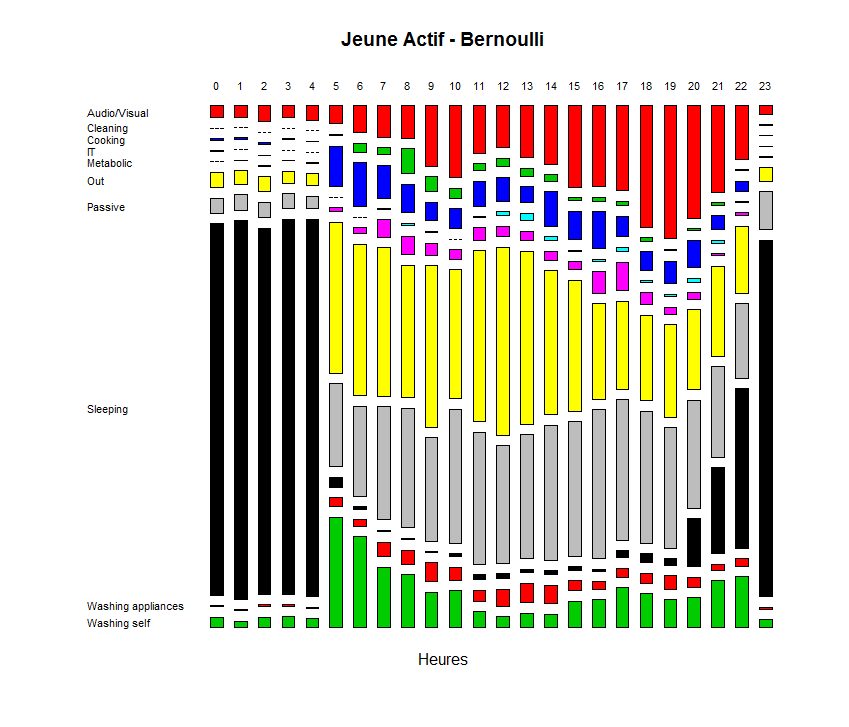
\includegraphics[scale=0.38]{Images/Activites/JeuneActifBernoulli} &
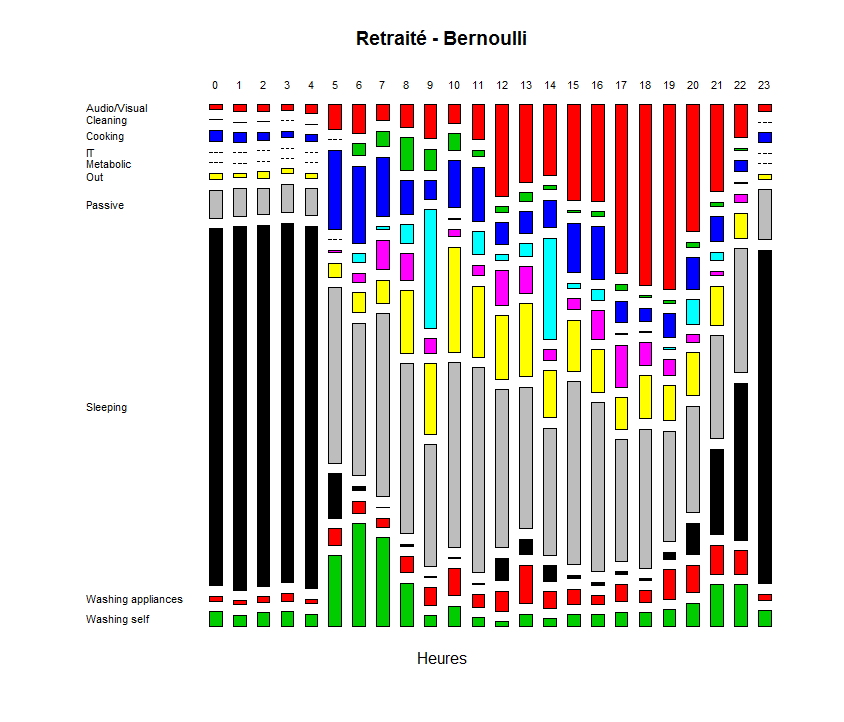
\includegraphics[scale=0.38]{Images/Activites/RetraiteBernoulli} \\
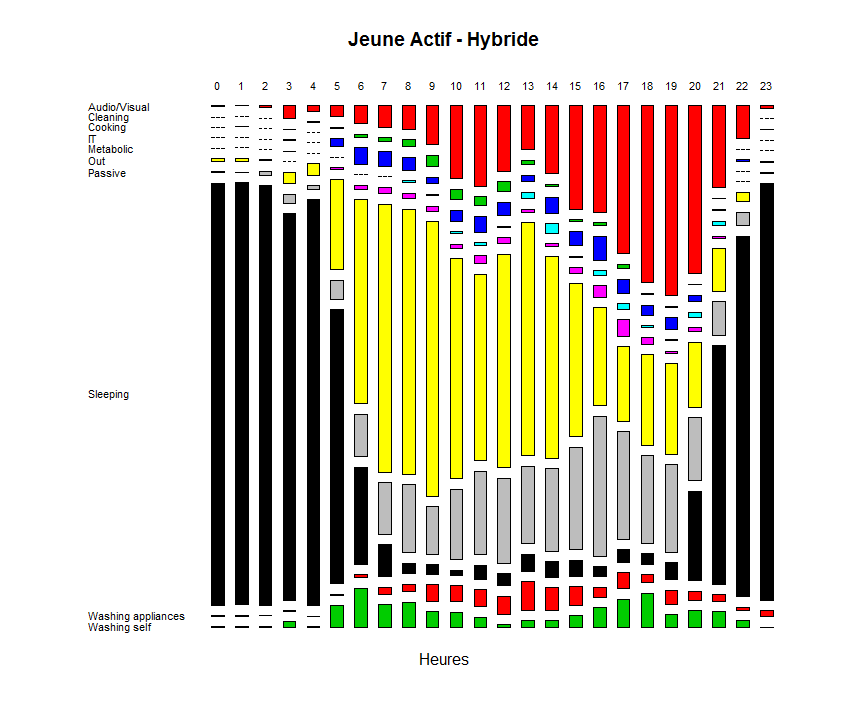
\includegraphics[scale=0.38]{Images/Activites/JeuneActifHybride} &
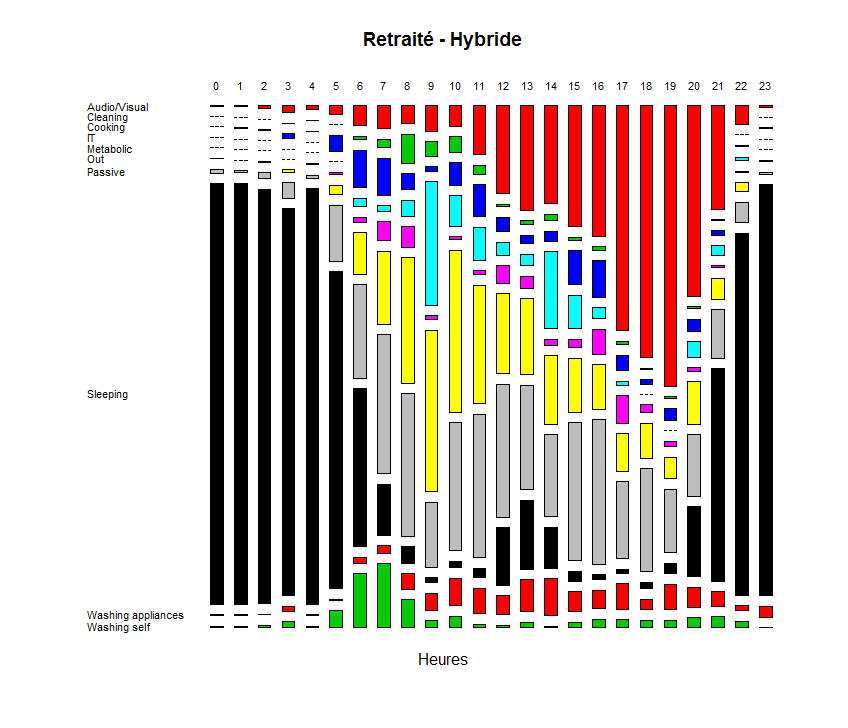
\includegraphics[scale=0.38]{Images/Activites/RetraiteHybride} \\
\end{tabular}
\caption{Chronogramme moyen des activités sur une journée calculé sur 150 jours, pour un jeune actif (à gauche) et pour un retraité (à droite), selon le modèle de Bernoulli (en haut) et le modèle hybride Bernoulli + Weibull(en bas), toutes choses égales par ailleurs}
\label{fig:Activités}
\end{figure}

\begin{figure}[H]
\centering
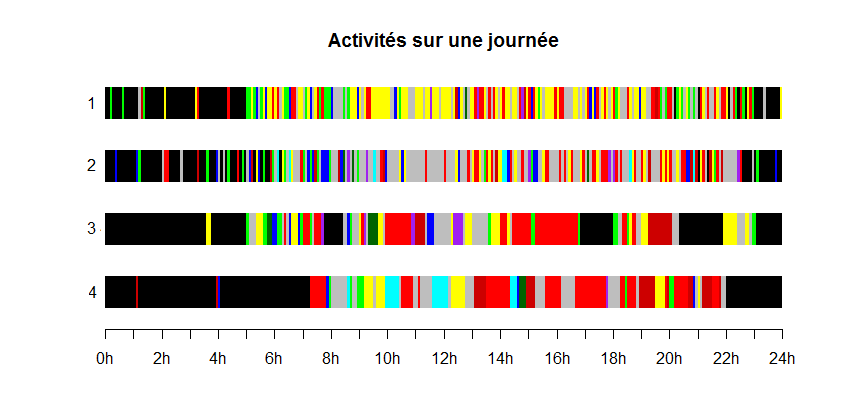
\includegraphics[scale=0.7]{Images/Activites/ActivitesSurUneJournee}
\caption{Exemple de scénarios d'activités pour une journée d'hiver pour; 1- l'ctif avec le modèle de Bernoulli, 2- le retraité avec le modèle de Bernoulli, 3- l'actif avec le modèle hybride, 4- le retraité avec le modèle hybride. Le code couleur est le même que pour la Figure \ref{fig:Activités}}
\label{fig:ExempleScenario}
\end{figure}

\section{Gestion des ouvrants}

1- Etat de l'art des modèles de gestion des fenêtres. Etudes sociologiques sur l'ouverture des fenêtres. Vérification du modèle utilisé par Schweiker et al. \cite{Schweiker-12}

2- Présentation du modèle courant 

3- Incorporation de phénomènes sociologiques qualitatifs au modèle:
    - Lorsque l'activité cuisine a lieu on ouvre la fenêtre
    - Lorsque l'occupant se réveille alors il ouvre la fenêtre
    
\section{Gestion des stores}

1- Etat de l'art sur les drivers de la gestion des stores
L'éblouissement est un driver important pour la gestion des stores. Néanmoins, l'éblouissement est difficilement exprimable numériquement il est donc peu évident de l'intégrer dans les outils de simulation.

2- Présentation du modèle courant

3- Incorporation de facteur contextuels qualitatifs au modèle:
	- Lorsque l'activité audio-visuelle a lieu on ferme les stores
	- Lorsque l'activité dormir a lieu on ferme les stores
	
\section{Gestion de l'éclairage}
\label{Gestion de l'éclairage}

1- Présentation du modèle courant

2- Incorporation de phénomènes sociologiques qualitatifs au modèle:
	- Lorsque l'activité audio-visuelle a lieu on ferme la lumière
	- Lorsque l'activité dormir a lieu on éteins forcément la lumière

\section{Utilisation des appareils électriques}

\subsection{Types d'appareils électriques}

Widén (2009) a catégorisé les appareils électriques en fonction de l'utilisation de la puissance:
\begin{table} [H]
\centering
\begin{tabular}{|l||l|}
Type de puissance & Exemple \\
\hline
\hline Puissance non définie par l'activité & Appareils de froid, radio réveil \\
\hline Puissance constante pendant l'activité & Télévision, Appareils de cuisson \\
\hline Puissance constante après l'activité & Machine à laver, lave vaisselle \\
\hline Puissance constante après avec contrainte de temps & Bains, douches \\
\hline Activité avec puissance dépendante du temps & Éclairage (variations journalières et de saison) \\
\hline 
\end{tabular}
\end{table}
Une catégorisation de la sorte permet une étude temporelle de la variation d'énergie.

\subsection{Modélisation de la possession et de l'utilisation des appareils électriques}

Jaboob (2015) propose une modélisation du taux de pénétration \footnote{Le taux de pénétration aussi appelé taux d'équipement est le pourcentage de la population équipée d'un appareil électrique}de la possession, de l'utilisation et de la fraction de puissance des appareils électriques. Cette modélisation est de type bottom-up pour chaque famille d'appareil, cela permet de considérer la diversité des ménages, des comportements individuels des occupants et bien sûr les caractéristiques intrinsèques des appareils. La modélisation de la possession des appareils est réalisée par régression logistique. La modélisation de l'utilisation des appareils considère d'une part l'allumage et d'autre part sa durée d'utilisation. L'allumage est modélisé par Bernoulli et la durée par un processus aléatoire à temps continu. La modélisation de la fraction de la puissance est réalisée par processus de Bernoulli ou de Markov.

\section{Gestion des consignes de température}

1- Que cherche t-on? Prédire la température de consigne pour l'envoyer au cœur de calcul.

2- Introduction sur le choix de la température de chauffage (Brisepierre, p273 - sociologie de l'energie]

3- Comment la température de consigne est utilisée par EnergyPlus? En étudiant la température intérieure on s'aperçoit qu'elle est strictement égale à la température de consigne. Hypothèse également faite par le CEREMA dans ces travaux sur le suivi de bâtiments démonstrateurs à basse consommation. (p127  Bat démonstrateurs à basse consommation d'énergie - Enseignements opérationnels tirés de 60 constructions et rénovations du programme PREBAT 2012-2015). "L'analyse statistique des températures en période de chauffe permet d'estimer la température en hiver en se basant sur la mesure de la température intérieur pendant les heures de fonctionnement du chauffage et pendant les heures d'occupation identifiées par enquête."

4- Quels sont les facteurs influençant l'utilisation des systèmes de chauffage.

Plusieurs études ont recensé les facteurs influençant l'utilisation des systèmes de chauffage. L'Annex53 \cite{Annex-53-1} a synthétisé l'ensemble de ces facteurs d'un point de vu qualitatif. Maresca et al. \cite{Maresca-09} ont pour leur part réalisé une étude pour le compte du CREDOC sur la maîtrise des consommations d'énergie des ménages. L'approche sociologique par plan d'expérience est pleine d'enseignements, cette approche permet notamment de déterminer avec un minimum d'essai l'influence individuel des différents paramètres. Dealière et al \cite{Devaliere-11} dans l'article de l'INSEE - La précarité énergétique: avoir froid ou dépenser trop pour se chauffer - justifient les différences de satisfaction thermique selon des variables propres au ménage, comme le revenu et sa structure, mais également par la vétusté du logement et le système de chauffage. Cavailhes et al.\cite{Cavailhes-11} de l'INRA  ont utilisé des méthodes d'économétrie de données de panel issues des enquêtes logement de l'INSEE. Cette étude considère l'ensemble des variables explicatives généralement avancé mais présente ses résultats sous forme d'évolution entre les années de référence de l'étude, 1984 et 1988, ce qui les rend difficilement exploitable dans notre contexte. Penot-Antoniou et al. \cite{Penot-Antoniou-13} dans le rapport sur les déterminants de la température de chauffage, analysent la variance entre la température adoptée par les ménages et les variables explicatives qualitatives. L'approche est celle qui correspond au besoin, car elle laisse la possibilité d'être codé et intégré à notre plateforme comportementale, en revanche un certain nombre de paramètres issus de l'étude économétrique ont des coefficients difficilement explicables. Par exemple un ménage ayant des ressources comprises entre 535 et 1100 \euro se chauffe de 2.5 \degre C de plus que la moyenne alors qu'un ménage gagnant de 1100 à 1500 \euro se chauffe moins de 1.7 \degre C en moyenne. Ce résultat non linaire n'est pas une exception et soulève un doute sur la fiabilité de l'étude, qui se repose pourtant sur un échantillon de 373 ménages.

\cite{Kelly-13} : Complexe mais parcimonisation envisageable

\cite{Andersen-09} : Petite étude sur 13 logements

\cite{Fabi-13}: Même données qu'Andersen mais développement d'un modèle logistique plutôt que linéaire.


\begin{table} [H]
\centering
\begin{tabular}{|l||c|c|c|c|c|c|c|}
\hline
\textbf{Littérature} & \cite{Annex-53-1} & \cite{Maresca-09} & \cite{Devaliere-11} & \cite{Cavailhes-11} & \cite{Penot-Antoniou-13} & \cite{Kelly-13} & \cite{Andersen-09} \\
\hline
\hline \rowcolor{gray}\textbf{Variables in-transmutables} & & & & & & & \\
\hline Zone climatique & & & & X & X & & \\
\hline Température extérieure & X & & & & & X & X \\
\hline Humidité relative / Pluie & X & & & X & & & X \\
\hline Altitude & & & & X & & & \\
\hline Vitesse du vent & X & & & & & & X \\
\hline Radiation solaire & & & & & & & X \\
\hline Localisation / Type de commune & & X & & X & & X & \\
\hline Heure de la journée & X & & & & & & X \\
\hline \rowcolor{gray} \textbf{Variables comportementales et \newline socio-démographiques} & & & & & & & \\
\hline Statut d'occupation & X & & X & X & X & X &  \\
\hline Revenu & & X & X & & X & X & \\
\hline Age & & X & & X & X & X & \\
\hline Nationalité & & & & X & & & \\
\hline Diplôme & & & & X & & & \\
\hline Genre & X & & & X & & & \\
\hline Coût du chauffage & & & X & X & & & \\
\hline Structure du ménage / CO2 & & & X & & X & X & X \\
\hline Vêture & X & & & & & & \\
\hline Stratégie de régulation & X & & & & & X & \\
\hline \rowcolor{gray}\textbf{Variables bâti et systèmes} & & & & & & & \\
\hline Année de construction & & X & X & X & X & X & \\
\hline Travaux de réhabilitation & & & & & X & & \\
\hline Type de chauffage & & & X & X & X & X & \\
\hline Type de combustible & & & & & X & X & \\
\hline Qualité enveloppe & X & & X & X & X & X & \\
\hline Structure du bâti (individuel/collectif) & & X & X & & & X & \\
\hline Exposition principale & & & & X & & & \\
\hline Superficie & & X & & X & & & \\
\hline Étage & & & & X & & & \\
\hline Pièces du logement & & X & & & & & \\
\hline Type de ventilation & X & & & & & & \\
\hline 
\end{tabular}
\end{table}

D'autres modèles ont été développé comme l'analyse statistique de Karjalainen -----CITE----- sur l'utilisation des thermostats en Finlande ou la régression linéaire multivariée de Schweiker et al. sur la modélisation de l'air conditionné au Japon... <- T. Hong, An Ontology to represent energy ....

Notre choix se porte sur le modèle de Kelly et al. car il est basé sur une étude significative, car ...

5- Choix pour le modèle de Kelly. Avec adaptation pour un modèle plus parcimonieux.

Pour développer un modèle, de type régression linéaire multiple, un logiciel de programmation statistique - comme R - a été utilisé. Ce type de logiciel permet de déterminer les coefficients Alpha et $a_{i}$ de l'équation de régression:

\begin{equation}
T_{int} = Alpha + \sum\limits_{i=1}^n a_{i} * V_{i} 
\end{equation}

Avec $T_{int}$ la température intérieure journalière, $Alpha$ et $a_{i}$ les coefficients à déterminer pour la régression et $V_{i}$ les valeurs des variables explicatives.

Pour obtenir les différents coefficients sous R il suffit de rentrer la fonction lm() en y spécifiant la variable à expliquer, les variables explicatives et la localisation du fichier:
\begin{verbatim}
   lm(Tint ~ Text + Text2 + Localisation + ... + Dbl_Glz + Wall_U, data = mydata)
\end{verbatim}

Le logiciel R génère alors les coefficients de la régression et 

Au risque de 1\%, il n'existe pas d'association statistiquement significative entre la température intérieure et les variables explicatives: déclaration de température de consigne, présence d'un programmateur automatique, tranche d'age de 60-64 ans, présence d'un système de chauffage central et d'un système de chauffage au gaz d'appoint. Ces variables explicatives sont donc supprimées du modèle développé.

Nous proposons aussi dans le fichier de configuration de laisser la possibilité aux utilisateurs de ne pas définir certains paramètres lorsqu'ils ne sont pas connus!

6- Changement de la température intérieure

\cite{Fabi-13}
Le modèle résulte en de petits ajustements de la température de consigne. Cela est en adéquation avec les résultats de l'étude d'Andersen \cite{Andersen-09} qui indique que les actions adaptatives des habitants lorsqu'ils ont froid sont de 66 à 78 \% du temps de petits ajustement contre moins de 5\% du temps des grosses augmentations sur le thermostat.

7- Interactions sociales ...

Le modèle de base de Kelly peut être complété par l'incorporation d'informations qualitatives supplémentaires

La température de consigne fixée à 19 \degre C depuis le choc pétrolier de 1974 fait figure de norme mais ne reflète pas les faits réels. Son influence sur les consommations énergétiques y est très fortement corrélé et un ajustement plus fidèle à la réalité est nécessaire.
Pour cela le modèle proposé consiste à tirer sur une loi normale la température de base issue du bureau d'études d'Enertech. Puis, en fonction des paramètres d'influences V (age, genre, charge financière, zone, longue absence...) la base est modifiée:

\[T_{consprinc}=T_{base}+\sum_{V}X_{V}\]

Cette approche proposée par Vorger \cite{Vorger-14} est très souple et permet notamment de gérer les réduits. Son calibrage est néanmoins discutable car basé sur le bon sens. En ce basant sur le \textit{British Home Heating Study} qui a réalisé une enquête sur les systèmes de chauffage et de contrôle, un modèle sur le choix de la température de consigne, notamment en fonction du systèmes, peut être créé plus finement. Cette enquête est composée d'un questionnaire et de mesures dynamiques (températures, humidité relative, ...) sur un échantillon de 32 familles anglaises.

Manque de données nous oblige à adopter une approche empirique, plutôt que de ré-exploiter des modèles qui ne nous semble pas robustes. Le modèle proposé a donc vocation à être amélioré, lorsque des données sur la fréquence des interactions des occupants avec le système de chauffage seront disponibles.



\section{Consommations d'eau chaude sanitaire}

\subsection{Systèmes}

Le modèle d'ETI ainsi que des données nationales (A trouver INSEE) peut permettre de modéliser les systèmes de chauffage de l'eau et le taux de pénétration des systèmes. Cette modélisation préalable est souvent omise dans les modèles de puisages d'ECS alors que son impacte sur les consommations finales en dépend relativement significativement.

On recense trois principales énergies pour la production d'eau chaude sanitaire: le gaz, l'électricité et les énergies renouvelables. Les chauffes-eau au gaz et électriques sont soit instantanés soit à accumulation. Concernant les énergies renouvelables, on retrouve de manière croissante le ballon thermodynamique ou pompe à chaleur et le chauffe eau solaire d'appoint.

\subsection{Volumes de consommation}

Selon Evarts et Swan \cite{Evarts-13} les puisages d'ECS sont très diverses selon les ménages et donc dépendent de leurs caractéristiques socio-démographiques. La fréquence et l'intensité des puisages sont encore plus fortement corrélés aux activités des occupants.

Selon les activités en cours, des puisages d'ECS y sont associés. A titre d'exemple, l'activité nettoyage corporelle implique un puisage en lien avec celui de la douche ou du bain.

L'ADEME a lancé un programme de recherche, baptisé PACTE, pour améliorer l'efficacité énergétique de l'ECS dans l'habitat. Ces travaux visent à améliorer la prise en compte de la dimension socio-comportementale de l'usage de l'ECS et à modéliser, simuler et évaluer le fonctionnement des équipements. La figure \ref{fig:PACTEECS} présente les partenaires du PACTE ECS, dont l'investissement est de plus 8 millions d'euros sur 5 ans.

\begin{figure}[h]
\centering

\includegraphics[scale=0.8]{Images/PACTEECS}
\caption{Les différents partenaires du PACTE ECS}
\label{fig:PACTEECS}
\end{figure}

La figure \ref{fig:Foisonnement_ECS} révèle la diversité de consommation à l'échelle du logement plutôt qu'à celle d'un immeuble.

\begin{figure}[h]
\centering
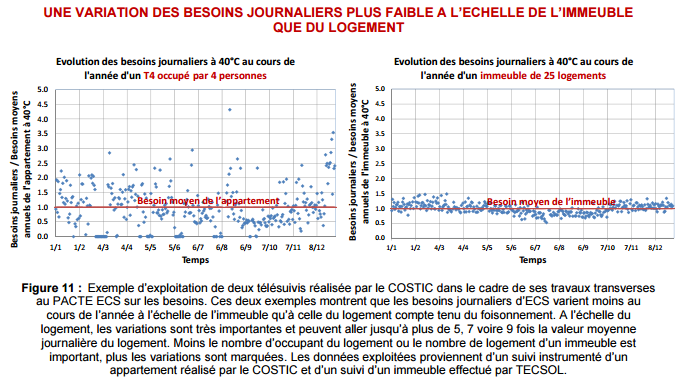
\includegraphics[scale=0.9]{Images/Foisonnement_ECS}
\caption{Importance de l'information à l'échelle du logement pour prendre en compte la diversité des consommations}
\label{fig:Foisonnement_ECS}
\end{figure}

La publication ADEME-COSTIC des résultats valorisés est prévue courant 2016 alors que l'étude se tient depuis 2011.

Contacter le directeur technique de COSTIC: Cedric Beaumont (prestations@costic.com) pour récupérer les résultats non agrégés 
